\documentclass[10pt,xcolor=dvipsnames]{beamer}
\usetheme{Madrid}
\usecolortheme[RGB={0,82,155}]{structure}
\setbeamertemplate{navigation symbols}{}

\usepackage[utf8]{inputenc}
\usepackage[spanish]{babel}
\usepackage{amsmath,amssymb}
\usepackage{hyperref}
\usepackage{tikz}
\usetikzlibrary{arrows.meta}
\usepackage{booktabs}
\setbeamerfont{caption}{size=\tiny}
% Bundled vector PDFs: no Mayan/Egyptian Unicode font needed at runtime.
\newcommand{\mayaicon}[1]{\raisebox{-0.32\height}{\includegraphics[width=0.47cm]{images/maya_vector/maya_#1.pdf}}}
\newcommand{\egypticon}[1]{\raisebox{-0.3\height}{\includegraphics[width=0.65cm,height=0.40cm,keepaspectratio]{images/egyptian/#1.pdf}}}

\title[Sistemas Numéricos]{Matemáticas Prehistóricas y Precolombinas}
\subtitle{Historia de la Matemática --- MM-517}
\author{}
\institute[UNAH]{Universidad Nacional Autónoma de Honduras \\ Facultad de Ciencias \\ Departamento de Matemáticas}
\date{III Período, 2026}

\AtBeginSection[]{%
  \begin{frame}<beamer>\frametitle{Contenido}
    \tableofcontents[currentsection]
  \end{frame}
}

\begin{document}

\begin{frame}
  \titlepage
\end{frame}

%% ======================================================================
\section{Sistemas numéricos en la prehistoria}
%% ======================================================================

\begin{frame}{Paleolítico Superior: el origen del conteo}
   
    \begin{columns}
        \begin{column}{0.6\textwidth}
  \begin{itemize}
    \item Período: \textbf{Paleolítico Superior} (\textasciitilde 50{,}000--10{,}000 BCE)
    \item Notación más antigua: \textbf{muescas en hueso} (\textit{tally marks})
    \item \textbf{Hueso de Lebombo}: \textasciitilde 44{,}000 años
      \begin{itemize}
        \item Border Cave (Sudáfrica)
        \item 29 muescas: posible calendario lunar
      \end{itemize}
    \item \textbf{Hueso de Ishango}: \textasciitilde 20{,}000 años
      \begin{itemize}
        \item Fíbula de babuino, RD Congo (descubierto 1960)
        \item Tres columnas de muescas: posible aritmética
      \end{itemize}
    \item Conteo corporal: bases 5 y 10
  \end{itemize}
        \end{column}
        \begin{column}{0.4\textwidth}
            \begin{figure}
                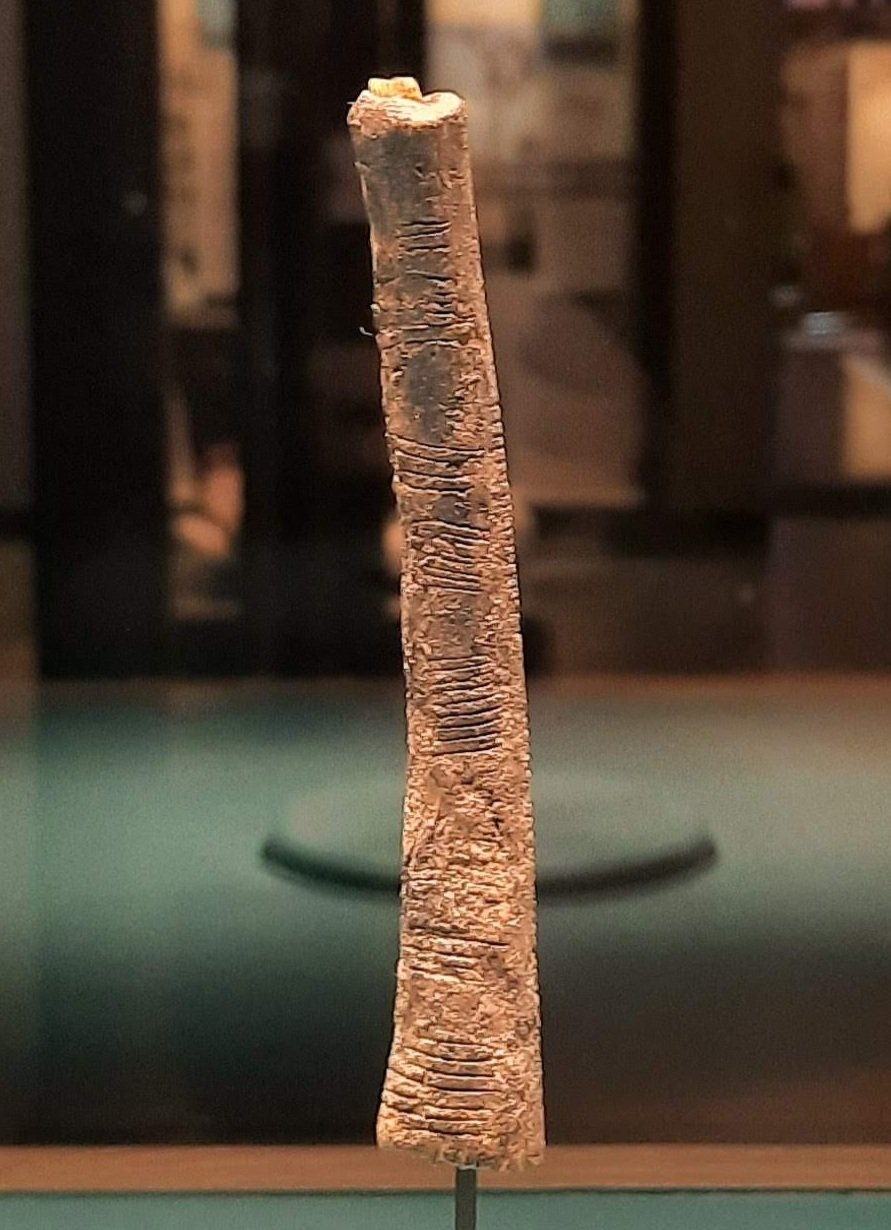
\includegraphics[width=0.9\textwidth]{images/Ishango_bone.jpg}
                \caption{Hueso de Ishango. By Joeykentin - \href{https://commons.wikimedia.org/w/index.php?curid=137144641}{Wikimedia Commons}}
            \end{figure}
        \end{column}
    \end{columns} 
\end{frame}


%% ======================================================================
\section{El período neolítico}
%% ======================================================================

\begin{frame}{Neolítico y casos clave (Ötzi, Egtved)}
  \begin{itemize}
    \item \textbf{Período Neolítico}: \textasciitilde 10{,}000--4{,}500 BCE (Cercano Oriente)
    \item \textbf{Ötzi el Hombre de Hielo}: \textasciitilde 3300 BCE (Edad del Cobre / Neolítico tardío)
      \begin{itemize}
        \item Hallado en los Alpes de Ötztal (Austria/Italia), 1991
        \item Hacha de cobre + herramientas de piedra
        \item Más antiguo que las pirámides egipcias y Stonehenge
      \end{itemize}
    \item \textbf{Niña de Egtved}: \textasciitilde 1370 BCE --- \textit{Edad del Bronce}
      \begin{itemize}
        \item Hallada en Dinamarca (1921); momificación en turbera
        \item Edad estimada: 16--18 años
      \end{itemize}
  \end{itemize}
  \begin{alertblock}{Nota}
    La Niña de Egtved pertenece a la \textbf{Edad del Bronce}, no al Neolítico estricto.
  \end{alertblock}
\end{frame}

\begin{frame}{Imágenes y nota}
   
    \begin{columns}
        \begin{column}{0.5\textwidth}
            \begin{figure}
                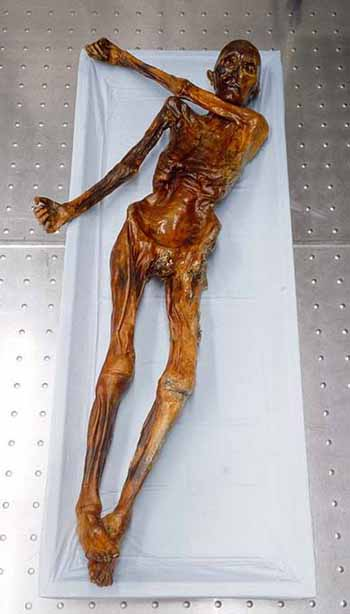
\includegraphics[width=0.9\textwidth,height=5.9cm,keepaspectratio]{images/otzitable.jpg}
            \end{figure}
        \end{column}
        \begin{column}{0.5\textwidth}
            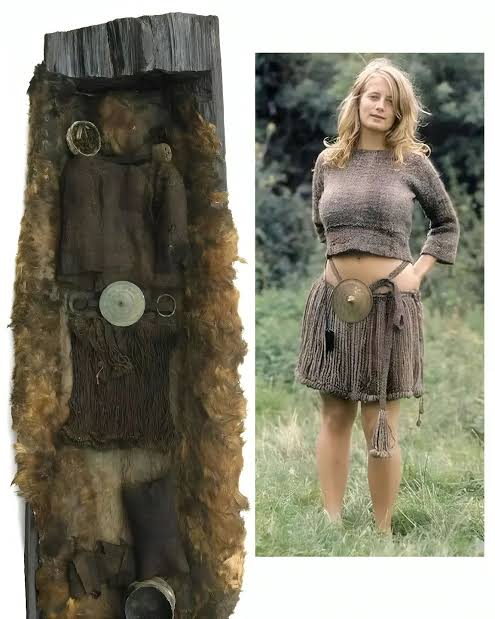
\includegraphics[width=0.9\textwidth,height=5.9cm,keepaspectratio]{images/etgved.jpeg}
        \end{column}
    \end{columns} 
\end{frame}

%% ======================================================================
\section{Matemáticas del Neolítico}
%% ======================================================================

\begin{frame}{¿Qué matemáticas se hacían?}
  \begin{itemize}
    \item \textbf{Sin escritura} ni notación simbólica formal
    \item Herramientas principales:
      \begin{itemize}
        \item Cuerdas con nudos
        \item Muescas en palos y huesos (\textit{tally sticks})
        \item Marcas en cuevas y megalitos
      \end{itemize}
    \item \textbf{Observación astronómica}:
      \begin{itemize}
        \item Ciclos lunares (29 días)
        \item Equinoccios y solsticios
      \end{itemize}
    \item \textbf{Geometría práctica}:
      \begin{itemize}
        \item Stonehenge (\textasciitilde 3000--2000 BCE): alineamientos a solsticios; posible calendario solar de 365.25 días
        \item Triángulos pitagóricos (3-4-5, 5-12-13) en megalitos
      \end{itemize}
  \end{itemize}
\end{frame}

\begin{frame}{Artefactos y geometría}
  \vspace{0.1cm}
  \begin{center}
    \begin{figure}
  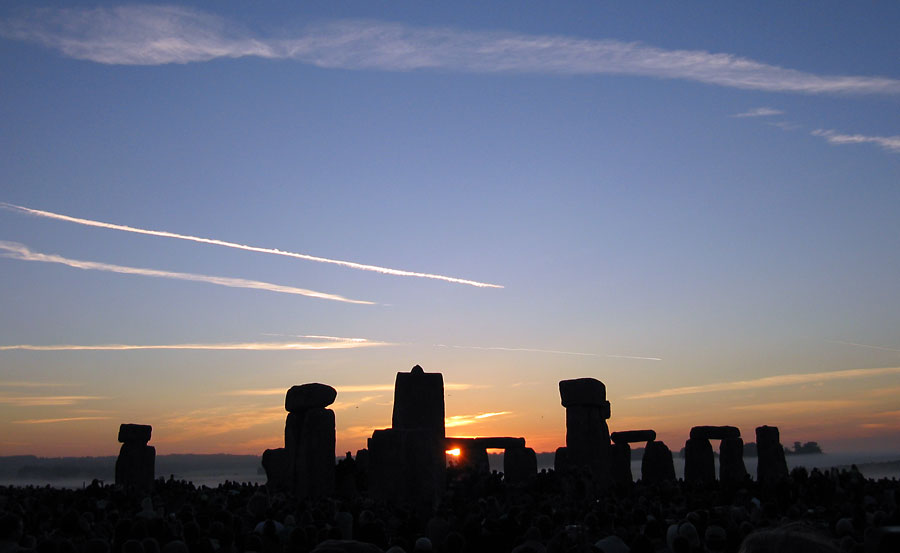
\includegraphics[width=0.85\textwidth,height=4.7cm,keepaspectratio]{images/stonehenge_solstice.jpg}
  \caption{Stonehenge al amanecer del solsticio de verano (21 jun 2005), alineación solar. By Andrew Dunn - \href{https://commons.wikimedia.org/wiki/File:Summer\_Solstice\_2005\_Sunrise\_over\_Stonehenge\_01.jpg}{Wikimedia Commons}}
\end{figure}
  \end{center}
\end{frame}

%% ======================================================================
\section{Sistema posicional babilónico}
%% ======================================================================

\begin{frame}{Sexagesimal y cuneiforme}
  \begin{itemize}
    \item \textbf{Origen}: Sumerios (\textasciitilde 3500--3000 BCE), Mesopotamia
    \item \textbf{Sistema sexagesimal} (base 60)
    \item \textbf{Escritura cuneiforme} sobre tablillas de arcilla
    \item \textbf{Posicional}: el valor depende de la posición
    \item Sub-base 10: dígitos 1--9 (cuñas) y 10 (esquina)
    \item Sin cero (espacio en blanco)
    \item \textbf{Períodos}:
      \begin{itemize}
        \item Sumerio: 3500--2000 BCE
        \item Babilónico antiguo: 2000--1595 BCE
        \item Babilónico nuevo: 1595--1155 BCE
        \item Seleúcida: 312--63 BCE
      \end{itemize}
  \end{itemize}
\end{frame}

\begin{frame}{Tablillas famosas y legado moderno}
  \begin{itemize}
    \item \textbf{Plimpton 322} (\textasciitilde 1900--1600 BCE): triadas pitagóricas
    \item Tablillas de Senkerah: cuadrados hasta 59, cubos hasta 32
    \item Tablas de recíprocos, raíces cuadradas, ecuaciones
    \item \textbf{Legado moderno}:
      \begin{itemize}
        \item 60 segundos/minuto, 60 minutos/hora
        \item 360$^{\circ}$ por circunferencia
        \item Coordenadas geográficas (latitud/longitud)
      \end{itemize}
  \end{itemize}
  \vspace{0.3cm}
  \begin{center}
    \begin{figure}
  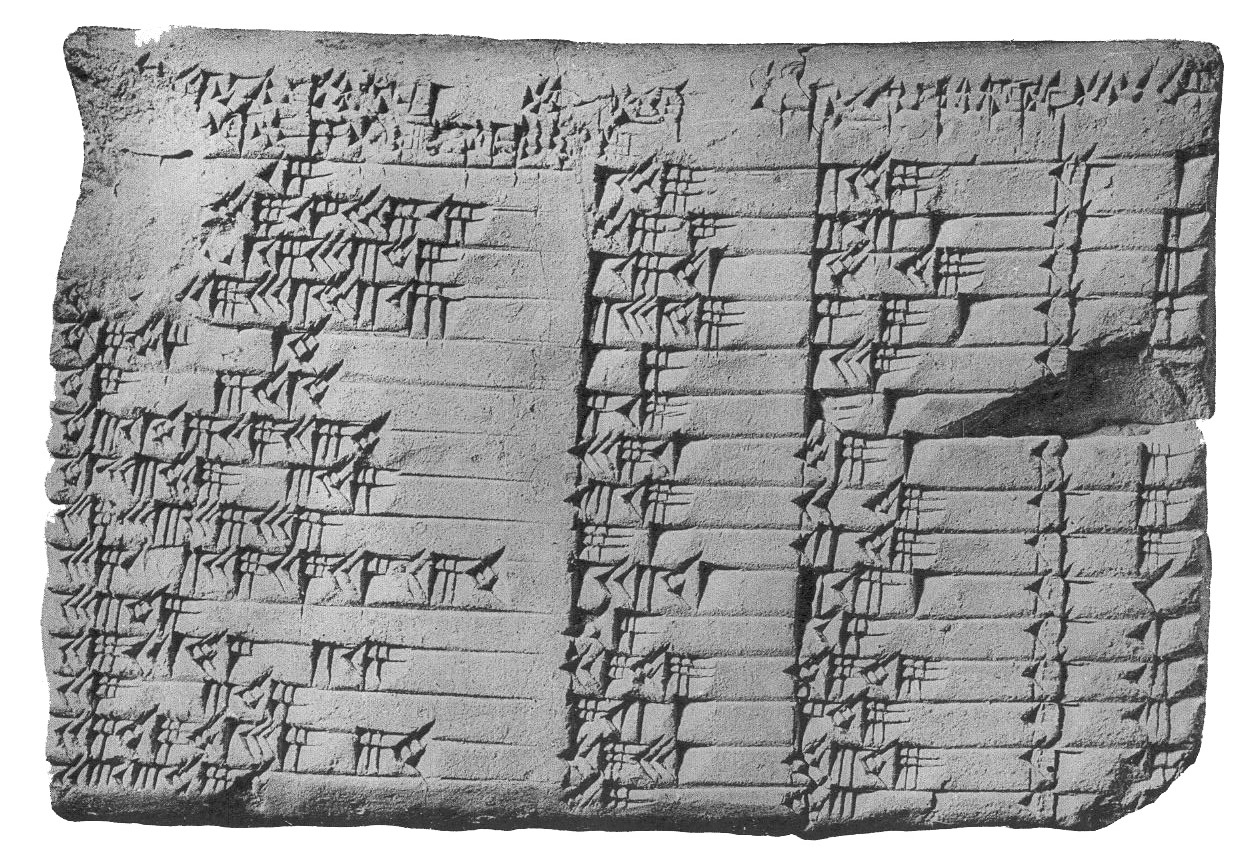
\includegraphics[width=0.55\textwidth,height=2.25cm,keepaspectratio]{images/plimpton_322.jpg}
  \caption{Tablilla Plimpton 322 (~1800 BCE): triadas pitagóricas en notación sexagesimal. By photo author unknown - \href{https://commons.wikimedia.org/wiki/File:Plimpton\_322.jpg}{Wikimedia Commons}}
\end{figure}
  \end{center}
\end{frame}

%% ======================================================================
\section{Numeración egipcia}
%% ======================================================================

\begin{frame}{Sistema jeroglífico}
  \begin{itemize}
    \item \textbf{Período}: \textasciitilde 3000 BCE -- 300 CE
    \item Sistema \textbf{decimal} (base 10)
    \item \textbf{Sin notación posicional}
    \item \textbf{Sin cero} (nfr $\neq$ cero matemático)
    \item \textbf{Símbolos jeroglíficos}:
      \begin{itemize}
        \item \makebox[0.8cm][c]{\egypticon{1-stroke}} 1 = trazo vertical
        \item \makebox[0.8cm][c]{\egypticon{10-cattle-hobble}} 10 = traba de ganado
        \item \makebox[0.8cm][c]{\egypticon{100-coil-rope}} 100 = espiral de cuerda
        \item \makebox[0.8cm][c]{\egypticon{1000-lotus}} 1{,}000 = flor de loto
        \item \makebox[0.8cm][c]{\egypticon{10000-finger}} 10{,}000 = dedo
        \item \makebox[0.8cm][c]{\egypticon{100000-tadpole}} 100{,}000 = renacuajo
        \item \makebox[0.8cm][c]{\egypticon{1000000-heh}} 1{,}000{,}000 = dios Heh
      \end{itemize}
    \item 9{,}999 necesitaba 36 símbolos (suma, no posición)
  \end{itemize}
  {\tiny Jeroglíficos: Otfried Lieberknecht, \href{https://commons.wikimedia.org/wiki/File:Num_aeg_hierog_0000001_L2R_80px.svg}{Wikimedia Commons},
  \href{https://creativecommons.org/licenses/by-sa/3.0/}{CC BY-SA 3.0}. Vectores, no fotografías.}
\end{frame}

\begin{frame}{Numeración hierática}
  \begin{itemize}
    \item Origen: \textasciitilde 3000 BCE; formalizada \textasciitilde 1800 BCE
    \item Usada en papiros: \textbf{Rhind} (\textasciitilde 1650 BCE), \textbf{Moscú} (\textasciitilde 1850 BCE)
    \item Versión cursiva de los jeroglíficos
    \item Coexistió con jeroglíficos por \textasciitilde 2000 años
    \item Seis formas históricas distintas (evolución)
  \end{itemize}
  \vspace{0.3cm}
  \begin{center}
    \begin{figure}
  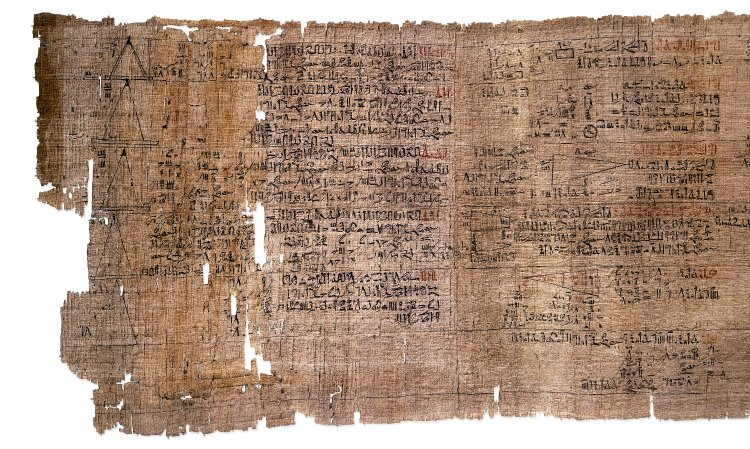
\includegraphics[width=0.55\textwidth,height=2.65cm,keepaspectratio]{images/rhind_papyrus.jpg}
  \caption{Papiro matemático Rhind (c. ~1650 BCE), detalle con numeración hierática. By Trustees of the British Museum - \href{https://commons.wikimedia.org/wiki/File:Rhind\_Mathematical\_Papyrus.jpg}{Wikimedia Commons}}
\end{figure}
  \end{center}
\end{frame}

%% ======================================================================
\section{Sistemas numéricos de América}
%% ======================================================================

\begin{frame}{Vigesimal y orígenes olmecas}
  \begin{itemize}
    \item \textbf{Origen}: cultura olmeca (\textasciitilde 1500--400 BCE), costa del Golfo de México
    \item \textbf{Base común}: vigesimal (base 20)
      \begin{itemize}
        \item Conteo con dedos de manos y pies
      \end{itemize}
    \item \textbf{Símbolos básicos}:
      \begin{itemize}
        \item \mayaicon{01} Punto = 1
        \item \mayaicon{05} Barra = 5
        \item \mayaicon{00} Concha = 0
      \end{itemize}
    \item \textbf{Culturas}:
      \begin{itemize}
        \item Olmeca (madre), Zapoteca (Monte Albán)
        \item Maya, Azteca, Mixteca
      \end{itemize}
    \item Calendario de Cuenta Larga: usado desde \textasciitilde 36 BCE
  \end{itemize}
  {\tiny Dibujos esquemáticos de los signos mayas; variantes históricas no representadas.}
\end{frame}

\begin{frame}{Mapa cronológico}
  \vspace{0.1cm}
  \begin{center}
    \begin{figure}
        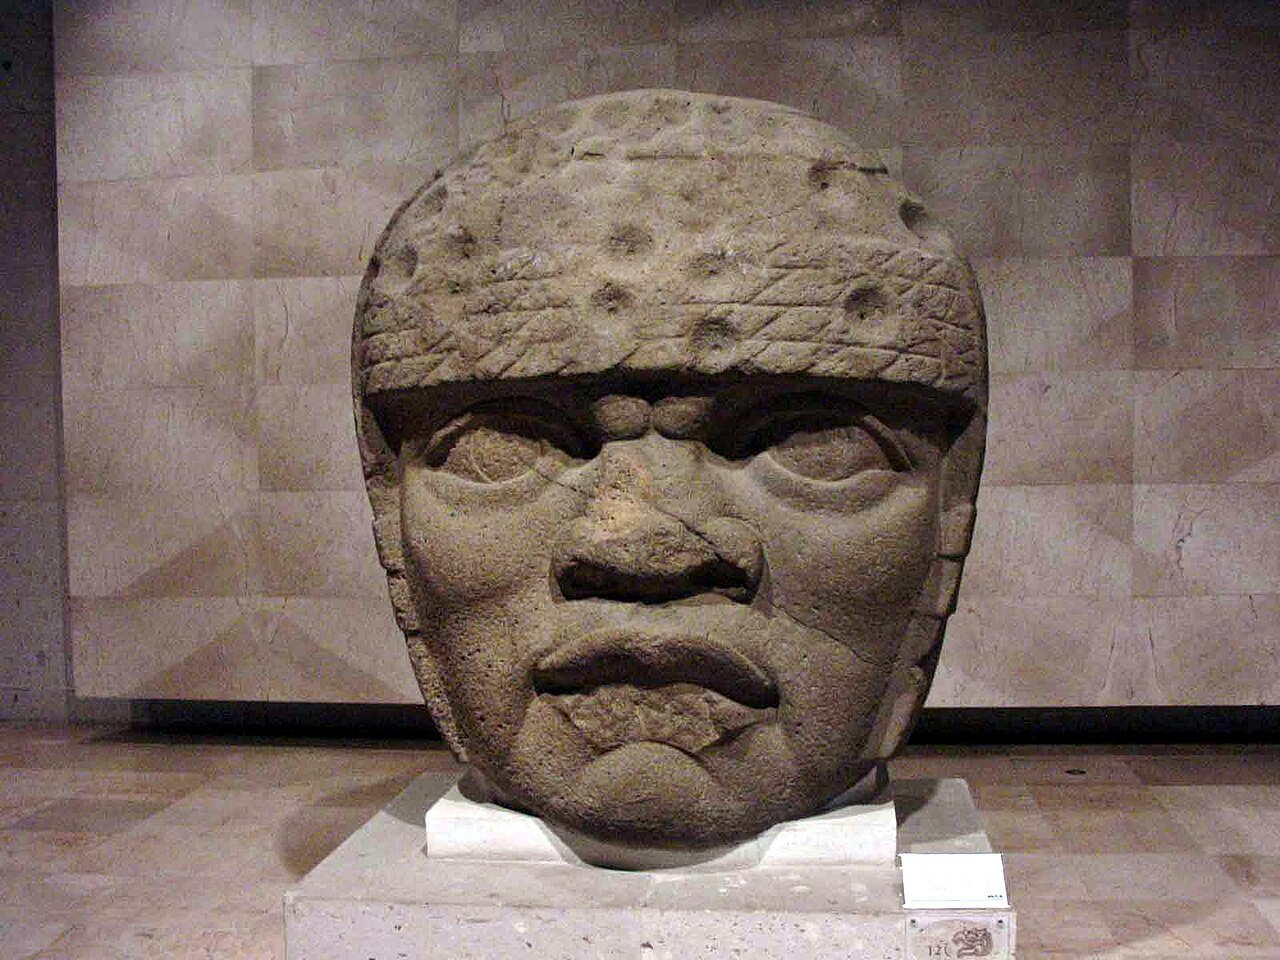
\includegraphics[width=0.85\textwidth,height=4.8cm,keepaspectratio]{images/olmeca1.jpg}
  \caption{Región cultural de Mesoamérica. By Alex Covarrubias - \href{https://commons.wikimedia.org/wiki/File:Region\_Mesoamerica.png}{Wikimedia Commons}}
\end{figure}
  \end{center}
\end{frame}

%% ======================================================================
\section{Sistema numérico y jeroglífico maya}
%% ======================================================================

\begin{frame}{Vigesimal posicional}
  \begin{itemize}
    \item \textbf{Período Clásico}: \textasciitilde 250--900 CE (sur de México, Guatemala, Belice)
    \item \textbf{Vigesimal} (base 20) posicional
    \item \textbf{Tres símbolos}:
      \begin{itemize}
        \item \mayaicon{00} Concha (o glifo de pétalo) = 0
        \item \mayaicon{01} Punto = 1
        \item \mayaicon{05} Barra = 5
      \end{itemize}
  \item \textbf{Posicional base 20}: 2$^{\circ}$ nivel es $18 \times 20 = 360$ (no $20 \times 20 = 400$), alineado con el año solar
    \item \textbf{Unidades temporales}:
      \begin{itemize}
        \item \textit{kin} = 1 día
        \item \textit{uinal} = 20 kin
        \item \textit{tun} = 18 uinal = 360 días
        \item \textit{katun} = 20 tun = 7{,}200 días
        \item \textit{baktun} = 20 katun = 144{,}000 días
      \end{itemize}
  \end{itemize}
  {\tiny Dibujos esquemáticos de los signos mayas; variantes históricas no representadas.}
\end{frame}

\begin{frame}{Calendarios y cero}
  \begin{columns}[T,onlytextwidth]
    \begin{column}{0.61\textwidth}
      \small
      \begin{itemize}
        \item \textbf{Tres calendarios}:
          \begin{itemize}
            \item \textit{Haab} (365 días, año vago)
            \item \textit{Tzolkin} (260 días, año sagrado)
            \item \textit{Cuenta Larga} (cronología absoluta)
          \end{itemize}
        \item \textbf{Cero matemático} usado desde \textasciitilde siglo III CE
        \item Primera fecha Cuenta Larga: \textbf{36 BCE} (Estela 2, Chiapa de Corzo; antecedente mesoamericano, no maya)
        \item Notación vertical u horizontal
      \end{itemize}
      \medskip
      \begin{beamercolorbox}[sep=5pt,rounded=true]{block body}
        \centering\scriptsize
        \textbf{El cero ocupa una posición}\par\smallskip
        
\includegraphics[width=0.67cm]{images/maya_vector/maya_13.pdf}\hspace{1pt}%
        
\includegraphics[width=0.67cm]{images/maya_vector/maya_00.pdf}\hspace{1pt}%
        
\includegraphics[width=0.67cm]{images/maya_vector/maya_00.pdf}\hspace{1pt}%
        
\includegraphics[width=0.67cm]{images/maya_vector/maya_00.pdf}\hspace{1pt}%
        
\includegraphics[width=0.67cm]{images/maya_vector/maya_00.pdf}\par
        $13.0.0.0.0$: fecha mítica de creación.\par
        {\tiny Esquema moderno, no calco de los glifos de la estela.}
      \end{beamercolorbox}
    \end{column}
    \begin{column}{0.36\textwidth}
      \centering
      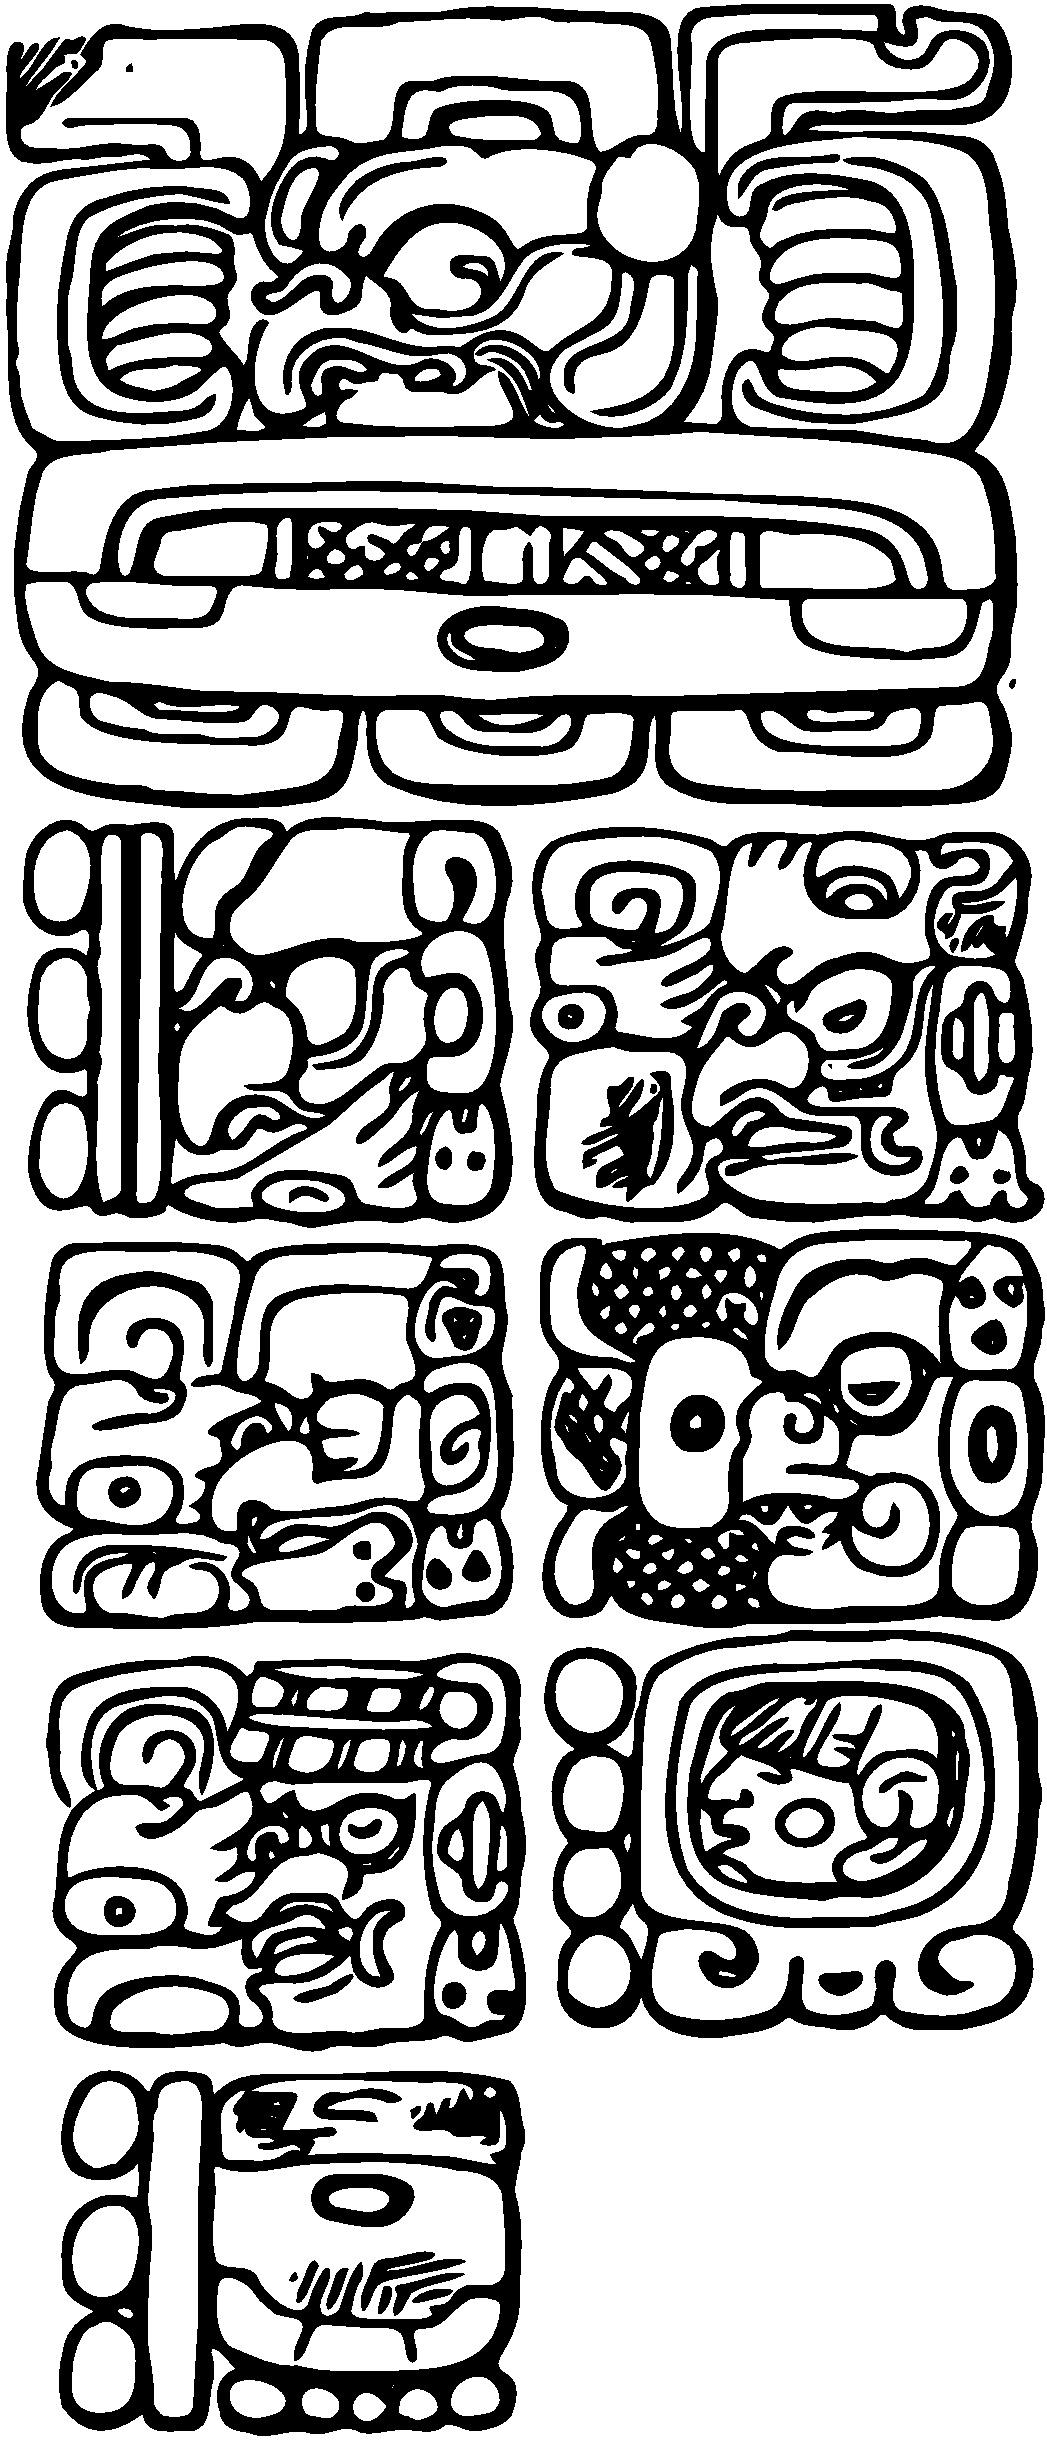
\includegraphics[width=\linewidth,height=4.65cm,keepaspectratio]{images/calendars/quirigua_stela_c.pdf}\par
      {\tiny Estela C de Quiriguá (Guatemala, 766 CE).\par
      Cara oriental: inscripción maya con la fecha mítica $13.0.0.0.0$.\par
      Dibujo: A. P. Maudslay; dominio público.\par
      \href{https://commons.wikimedia.org/wiki/File:East_side_of_stela_C,_Quirigua.svg}{Fuente: Wikimedia Commons}.}
    \end{column}
  \end{columns}
\end{frame}

%% ======================================================================
\section{Sistema azteca}
%% ======================================================================

\begin{frame}{Pictográfico vigesimal}
  \begin{itemize}
    \item \textbf{Imperio Mexica/Azteca (Triple Alianza)}: 1428--1521 CE
    \item \textbf{Vigesimal} (base 20) pictográfico
    \item \textbf{Símbolos}:
      \begin{itemize}
        \item Punto = 1
        \item Bandera / estandarte = 20
        \item Pluma = 400
        \item Bulto de copal = 8{,}000
      \end{itemize}
    \item \textbf{Uso}: tributos y registro comercial
    \item \textbf{Sin cero} explícito (a diferencia de Maya)
    \item Sistema \textbf{no posicional} estricto (suma)
  \end{itemize}
\end{frame}

\begin{frame}{Fuentes y comparación}
  \vspace{0.1cm}
  \begin{center}
    \begin{figure}
  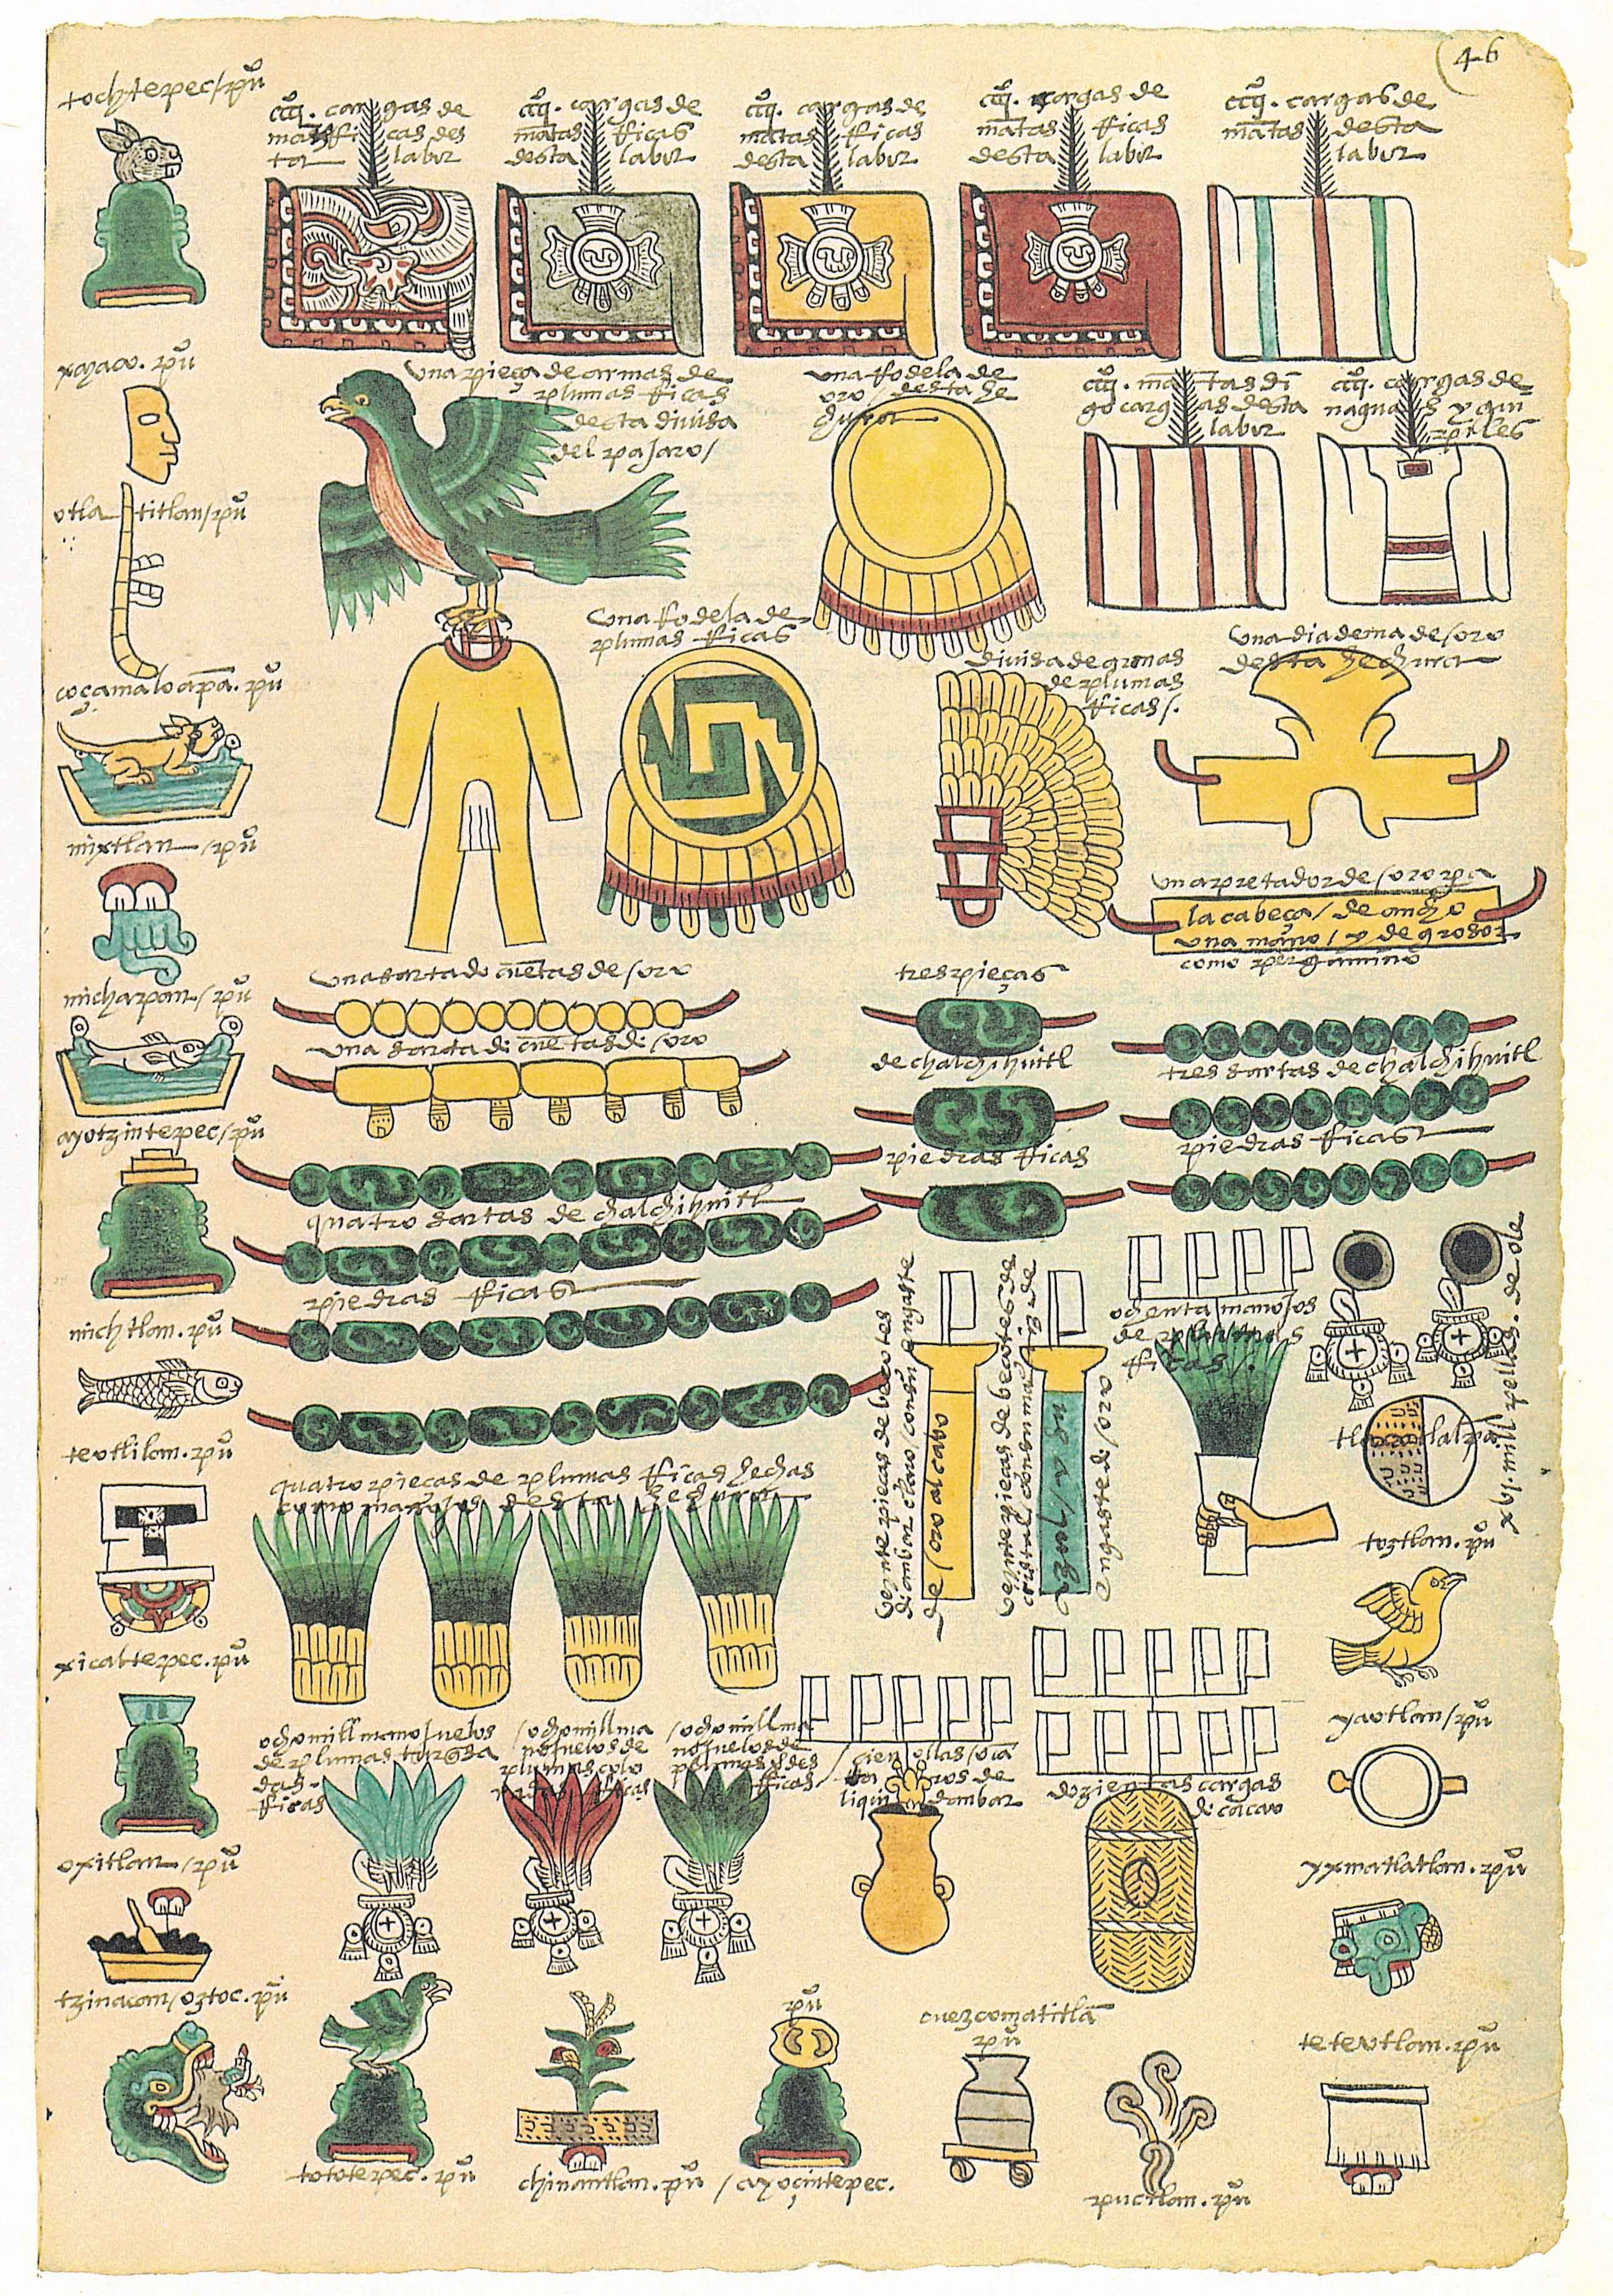
\includegraphics[width=0.85\textwidth,height=3.7cm,keepaspectratio]{images/codex_mendoza_46r.jpg}
  \caption{Códice Mendoza, folio 46r: tributos al imperio azteca. By El Comandante - \href{https://commons.wikimedia.org/wiki/File:Codex\_Mendoza\_folio\_46r.jpg}{Wikimedia Commons}}
\end{figure}
  \end{center}
  \vspace{0.2cm}
  \begin{alertblock}{Diferencia con Maya}
    Los aztecas \textbf{sumaban}; los mayas tenían notación \textbf{posicional} y usaban el \textbf{cero}.
  \end{alertblock}
\end{frame}

%% ======================================================================

\begin{frame}{Numerales mayas: 0--19}
  \begin{itemize}
    \item Unicode \textit{Mayan Numerals}: U+1D2E0--U+1D2F3 (0--19)
    \item Vectores locales: concha = 0, punto = 1, barra = 5
  \end{itemize}
  \begin{center}
  \setlength{\tabcolsep}{7pt}
  \begin{tabular}{ccccc}
    
\includegraphics[width=0.85cm]{images/maya_vector/maya_00.pdf}\,\textbf{0} & 
\includegraphics[width=0.85cm]{images/maya_vector/maya_01.pdf}\,\textbf{1} & 
\includegraphics[width=0.85cm]{images/maya_vector/maya_02.pdf}\,\textbf{2} & 
\includegraphics[width=0.85cm]{images/maya_vector/maya_03.pdf}\,\textbf{3} & 
\includegraphics[width=0.85cm]{images/maya_vector/maya_04.pdf}\,\textbf{4} \\[1pt]
    
\includegraphics[width=0.85cm]{images/maya_vector/maya_05.pdf}\,\textbf{5} & 
\includegraphics[width=0.85cm]{images/maya_vector/maya_06.pdf}\,\textbf{6} & 
\includegraphics[width=0.85cm]{images/maya_vector/maya_07.pdf}\,\textbf{7} & 
\includegraphics[width=0.85cm]{images/maya_vector/maya_08.pdf}\,\textbf{8} & 
\includegraphics[width=0.85cm]{images/maya_vector/maya_09.pdf}\,\textbf{9} \\[1pt]
    
\includegraphics[width=0.85cm]{images/maya_vector/maya_10.pdf}\,\textbf{10} & 
\includegraphics[width=0.85cm]{images/maya_vector/maya_11.pdf}\,\textbf{11} & 
\includegraphics[width=0.85cm]{images/maya_vector/maya_12.pdf}\,\textbf{12} & 
\includegraphics[width=0.85cm]{images/maya_vector/maya_13.pdf}\,\textbf{13} & 
\includegraphics[width=0.85cm]{images/maya_vector/maya_14.pdf}\,\textbf{14} \\[1pt]
    
\includegraphics[width=0.85cm]{images/maya_vector/maya_15.pdf}\,\textbf{15} & 
\includegraphics[width=0.85cm]{images/maya_vector/maya_16.pdf}\,\textbf{16} & 
\includegraphics[width=0.85cm]{images/maya_vector/maya_17.pdf}\,\textbf{17} & 
\includegraphics[width=0.85cm]{images/maya_vector/maya_18.pdf}\,\textbf{18} & 
\includegraphics[width=0.85cm]{images/maya_vector/maya_19.pdf}\,\textbf{19} \\[1pt]
  \end{tabular}\par\smallskip
  {\scriptsize Dibujos esquemáticos originales (CC0), no glifos de una fuente.\par
  \href{https://www.unicode.org/charts/PDF/U1D2E0.pdf}{Correspondencia de valores: tabla oficial de Unicode}.}
  \end{center}
\end{frame}

\section{Los quipus incas}
%% ======================================================================

\begin{frame}{Estructura y materiales}
  \begin{itemize}
    \item \textbf{Imperio Inca}: \textasciitilde 1438--1532 CE
    \item Uso más antiguo: \textasciitilde 2600 BCE (culturas andinas pre-Inca)
    \item \textbf{Cuerdas anudadas} (algodón o fibra de camélido: alpaca, llama, vicuña)
    \item \textbf{Información codificada}:
      \begin{itemize}
        \item Posición del nudo (decimal posicional)
        \item Color del cordón
        \item Tipo de nudo (simple, largo, en figura)
        \item Distancia entre nudos
        \item Orden de los cordones
      \end{itemize}
  \end{itemize}
\end{frame}

\begin{frame}{Uso, especialistas y escala}
  \begin{itemize}
    \item \textbf{Función principal}: numérica (decimal posicional)
    \item \textbf{Registros}: censos, tributos, calendario, producción, militar
    \item \textbf{Administradores}: \textit{quipucamayocs} (guardianes de la memoria)
    \item Estudios recientes sugieren posible contenido narrativo en algunos quipus
    \item \textbf{Escala}: desde pocos cordones hasta miles
  \end{itemize}
  \vspace{0.3cm}
  \begin{center}
    \begin{figure}
  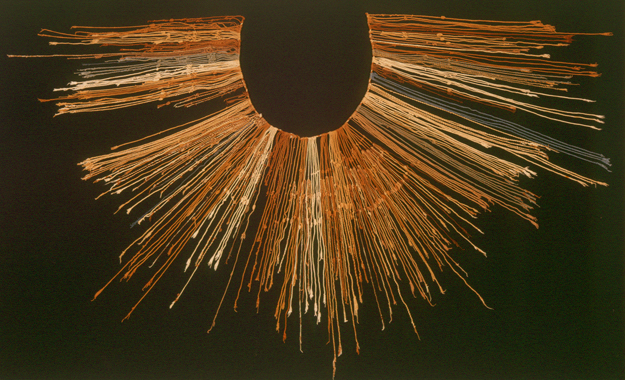
\includegraphics[width=0.55\textwidth,height=2.7cm,keepaspectratio]{images/quipu.jpg}
  \caption{Quipu inka del Museo Arqueológico Rafael Larco Herrera (Lima, Perú). By Museo Arqueológico Rafael Larco Herrera - \href{https://commons.wikimedia.org/wiki/File:Inca\_Quipu.jpg}{Wikimedia Commons}}
\end{figure}
  \end{center}
\end{frame}

\end{document}
